\documentclass[11pt,letterpaper]{article}

%% === basic packages ===
\usepackage{latexsym}
\usepackage{amssymb,amsmath}
\usepackage{graphicx}

%% === margins ===
\addtolength{\hoffset}{-0.75in} \addtolength{\voffset}{-0.75in}
\addtolength{\textwidth}{1.5in} \addtolength{\textheight}{1.6in}

%better PDF fonts
\usepackage{times}
\usepackage{mathptm}
\usepackage{amsfonts}

%% === bibliography packages ===
\usepackage{natbib}
\bibliographystyle{pa}

%% === hyperref options ===
\usepackage{color}
\usepackage[pdftex, bookmarksopen=true, 
bookmarksnumbered=true, linkcolor=webred]{hyperref}
\definecolor{webgreen}{rgb}{0, 0.5, 0}
\definecolor{webblue}{rgb}{0, 0, 0.5}
\definecolor{webred}{rgb}{0.5, 0, 0}

% === dcolumn package ===
\usepackage{dcolumn}
\newcolumntype{.}{D{.}{.}{-1}}
\newcolumntype{d}[1]{D{.}{.}{#1}}

% === theorem package ===
\usepackage{theorem}
\theoremstyle{plain} 
\theoremheaderfont{\scshape}
\newtheorem{definition}{Definition}
\newtheorem{assumption}{Assumption}
\def\qed{\hfill \vrule height7.5pt width6.17pt depth0pt}

% === rotate package ===
\usepackage{rotating}
\usepackage{longtable}

% === new commands ===
\newcommand\spacingset[1]{\renewcommand{\baselinestretch}%
  {#1}\small\normalsize}
\newcommand{\MC}{\multicolumn}
\newcommand{\Indep}{{\bot\negthickspace\negthickspace\bot}} 


\begin{document}

% bibtex citations to add when gkbibtex works again
%
%@article{koch:02,
%  author = {Koch, Jeffrey M.},
%  title =  {Gender Stereotypes and Citizens' Impressions of House
%  Candidates' Ideological Orientation},
%  journal = {American Journal of Political Science},
%  year =        {2002},
%  volume =    {46},
%  pages =     {453--462} 
%}
%
%@Book{popk:91,
%  author =       {Popkin, Samuel L.},
%  title =        {The Reasoning Voter: Communication and Persuasion in
%  Presidential Campaigns},
%  publisher =    {University of Chicago Press},
%  year =         {1991},
%  address =      {Chicago},
%}
%
%
%@Article{bart:96,
%  author =      {Bartels, Larry M.},
%  title =       {Uninformed Votes: Information Effects in Presidential Elections},
%  journal =     {American Journal of Political Science},
%  year =        {1996},
%  volume =      {40},
%  pages =       {194--230},
%}
%


% paste in from below here
\baselineskip=1.57\baselineskip

\section{Empirical Illustrations}

In this section, we provide empirical illustrations of how conceiving
of matching as preprocessing can reduce the sensitivity of inferences.
Social scientists are often faced with a perplexing array of
specification choices as discussed in Section~\ref{s:paraobs}.  Our
goal here is to demonstrate that matching as preprocessing has the
potential to reduce model sensitivity to such specification choices.
The result is that researchers may be able to estimate effects with
unjustified modeling assumptions playing a decreased role.  We define
sensitivity as the variability in point estimates across potential
specifications of pre-treatment covariates.  In these illustrations we
concern ourselves with bias, not efficiency, although the latter has
been the focus of much attention in the economic literature (cites). 

\subsection{Assessing the Causal Effect of Visibility on Candidate
  Evaluations}

In our first illustration we study citizen evaluations of ideological
position for candidates for the House of Representatives in the 1990s.
This data was first studied by \citet{koch:02} and we were able to
replicate substantially all of the results therein.\footnote{In our
  version of the dataset, political awareness is scaled slightly
  differently, a matter of no substantive significance that changes
  none of the results.  We thank Jeff Koch for providing the data and
  for clarifying this nominal difference.}  The treatment of interest
is the effect of being a highly visible female candidate on citizen
voter evaluations of the candidate's ideology (scored as a seven point
ordinal point scale,where high scores indicate greater
conservatism).\footnote{Visibility is measured originally by whether a
  candidate had campaign expenditures exceeding more than \$750,000.
  For simplicity and comparison to \citet{koch:02}, we do not concern
  ourselves here with the correctness of these measurements, nor do we
  seek to improve the methodology of studying an ordinal dependent
  variable.}  We confine ourselves to studying this effect on
Republican female candidates, compared to the control of invisible
male and female candidates.\footnote{This corresponds to the fourth
  column of Table 2 in \citet[p.  459]{koch:02}.}  Understanding the
micro-mechanisms of how citizens form impressions of candidates is of
great import to the literature on voting and information \citep[see,
e.g.,]{bart:96,popk:91}, yet field experiments that randomly assign
visibility to candidates are difficult to conduct for obvious reasons.

As a result, \citet{koch:02} collects observational data, including
potential confounding covariates of candidate ideology, voter
perception of party ideology, respondent ideology, feeling
thermometer, and political awareness.  Using ordinary least squares to
control for these covariates, the idea is that we can hold constant
all of these explanatory variables, varying only the treatment.  Yet,
we can quickly see that even with such a small number of covariates,
the curse of dimensionality looms large.  Given unique values of these
covariates, nonparametric estimation would require estimation of $4.4
\times 10^7$ parameters, yet the full dataset contains only 494 units.
So instead, \citet{koch:02} estimates the treatment effect by
assumption, employing ordinary least squares.

Yet as the first three columns in Table~\ref{tb:kochmtest} show,
visible and invisible female candidates differ drastically in
explanatory covariates.  Most strikingly, visible female candidates
tend to be substantially more liberal than invisible candidates:
visible candidates are rated 0.44 on a scale from 0 to 1, which is
almost one standard deviation higher than the 0.2 average rating of
invisible candidates (t-statistic=12.18).  In addition, visible
candidates appear to be slightly more politically aware
(t-statistic=2.42).  As a result of this covariate imbalance, we may
not be comfortable in reducing $4.4 \times 10^7$ parameters to 6
merely by assumption.  Indeed, model sensitivity may lead some
scholars to inadvertently report regressions that confirm some
hypotheses when other specifications would caution against such a
conclusion.  Merely six explanatory variables, for example, may enter
the right-hand side of a linear regression in 63 different ways
(=$\sum_{i=1}^6 {6 \choose i}$), but scholars rarely report results
across all such possible specifications.

\begin{table}[t]
  \begin{center}
    \begin{tabular}{lrrrrrr}
      \hline
      & \MC{3}{c}{\bf Raw Data} & \MC{3}{c}{\bf Pre-processed Data
      (subclass 4) }\\
      & Mean for  & Mean for  &    & Mean for  & Mean for \\
      & Treated & Control  & t-stat &    Treated & Control  & t-stat \\
      \hline
      Propensity Score & 0.48 & 0.10 & 10.71 & 0.61 & 0.54 & 2.32 \\
      Candidate Ideology & 0.44 & 0.20 & 12.18 & 0.50 & 0.48 & 1.15 \\
      Perception of Party Ideology & 0.72 & 0.73 & -0.42 & 0.69 & 0.67 & 0.24 \\
      Respondent Ideology & 0.49 & 0.53 & -0.97 & 0.45 & 0.50 & -0.38 \\
      \hspace{0.1in} Respondent Ideology $\times$ & 0.31 & 0.32 & -0.44 & 0.27 &
      0.25 & 0.18 \\
      Feeling Thermometer\\
      Feeling Thermometer & 0.60 & 0.55 & 1.70 & 0.54 & 0.53 & 0.03 \\
      Political Awareness & 0.76 & 0.70 & 2.42 & 0.76 & 0.74 & 0.28 \\
      \hline
    \end{tabular}
    \caption{Imbalance of pre-treatment covariates in the Koch data.
      The full sample size was 494, and the matched dataset with
      subclassification was 463.  The first three columns present
      means for visible (``treated'') and invisible (``control'')
      female Republican candidates and t-statistics for the full
      dataset.  The last three columns present means and t-statistics
      for one representative subclass.  This table shows that
      candidate ideology is highly imbalanced in the full Koch data,
      and that balance can be achieved by subclassification.  Visible
      females, for example, were much more likely to be perceived as
      liberal than invisible females overall, but within subclass 4
      this difference diminishes.}
    \label{tb:kochmtest}
  \end{center}
\end{table}

Preprocessing by matching reduces the imbalance of covariates so that
parametric assumptions play a smaller role in estimation.  We hence
match by subclassification on the propensity score.  The procedure is
quite simple, and easily implemented and further demonstrated in our
accompanying software and documentation.  (In addition, we investigate
other matching techniques, such as one-to-one nearest neighbor
matching and caliper matching, which yield the same substantive
results.)  We estimate the propensity score with a logistic
regression, using all six pre-treatment covariates as
predictors.\footnote{Throughout this application, we treat respondent
  ideology $\times$ feeling thermometer as one covariate as in
  \citet{koch:02}.}  We then discard treatment units whose propensity
score is greater than the maximum of control units and control units
whose propensity score is lower than the minimum of the treated units.
This results in 31 discarded units, and ensures that outliers do not
contaminate our data.  Next, we create 6 subclasses by quantiles of
the propensity score of the treated units.  As is desired, within each
subclass, covariate balance is substantially better than in the full
sample.  For example, the last three columns of
Table~\ref{tb:kochmtest} presents means and t-statistics for each
covariate in one representative subclass showing that balance
uniformly increases in each of these covariates.  Candidate ideology,
which was highly imbalanced in the raw data, is now 0.5 for visible
candidates within subclass 4, which differs only slightly from the
0.48 for invisible candidates in that subclass (t-statistic=1.15).

\begin{table}[t]
  \begin{center}
    \begin{tabular}{lrrrrrr}
      \hline
      & \MC{6}{c}{\bf Subclass} \\
      Covariate &  1 &  2 &  3 &  4 &  5 &  6 \\
      \hline
      Candidate Ideology & 2.16 & -0.85 & 0.33 & 1.15 & 1.51 & -0.45 \\
      Perception of Party Ideology & -0.65 & -1.05 & 0.59 & 0.24 & 0.06 & 1.53 \\
      Respondent Ideology & 1.45 & -0.73 & 1.08 & -0.38 & -1.26 & -1.00 \\
      Respondent Ideology $\times$ & 0.50 & -0.81 & 1.64 & 0.18 &
      -1.44 & -0.42 \\
      \hspace{0.1in} Feeling Thermometer \\
      Feeling Thermometer & -0.03 & 0.33 & 1.61 & 0.03 & -1.34 & 1.08 \\
      Political Awareness & 0.53 & 0.14 & -1.50 & 0.28 & -1.08 & 0.66 \\
      No. treated & 14.00 & 13.00 & 13.00 & 14.00 & 13.00 & 11.00 \\
      No. control & 299.00 & 30.00 & 39.00 & 12.00 & 3.00 & 2.00 \\
      $N$ & 313.00 & 43.00 & 52.00 & 26.00 & 16.00 & 13.00 \\
      \hline
    \end{tabular}
    \caption{Means test statistics for six pre-treatment covariates.
      Each cell presents t-statistic for the covariate within each
      subclass, and No. treated / control indicates the number of
      treated / control units in each subclass and $N$ indicates the total
      number of units in each subclass.  This table shows that
      relative balance can be achieved within each subclass with only
      six subclasses.}
    \label{tb:kochxsub}
  \end{center}
\end{table}

To check balance for all covariates in all of the subclasses,
Table~\ref{tb:kochxsub} presents simple means test statistics for each
of the main covariates in each of the subclasses.  The last three rows
present the number of unit in each subclass.  Note that there are few
visible candidates matched with many more invisible candidates in the
lower subclasses and the reverse in the higher subclasses.  Through
this simple technique we are able to compare relatively similar
candidates within each subclass.  Indeed across subclass-covariates
the t-statistic exceeds 2 only once, which is roughly the same as we
would expect if the data were generated randomly.

\begin{figure}[t]
  \spacingset{1} 
  \begin{center}
    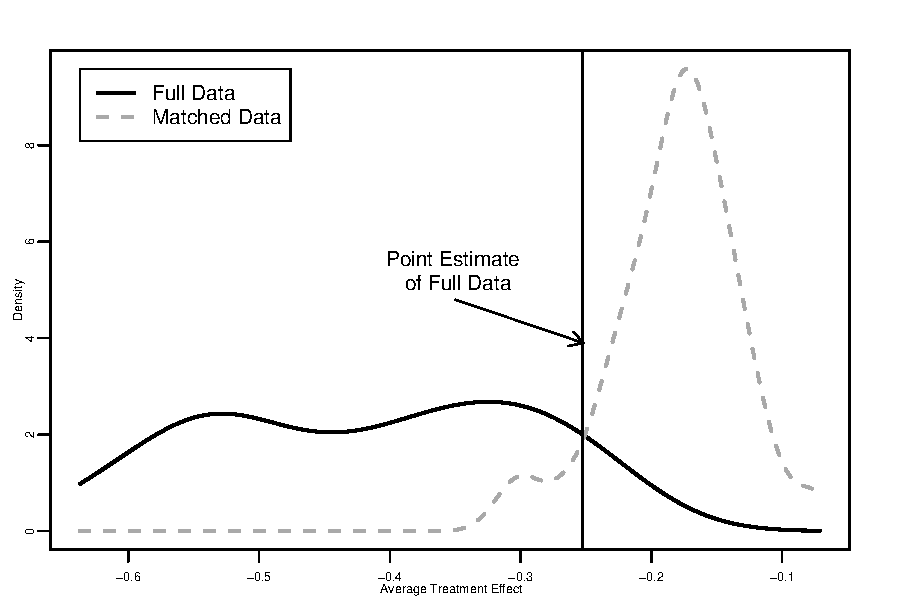
\includegraphics[height=3.5in,angle=0]{dens.pdf}
  \end{center}
  \vspace{-0.275in}
  \caption{Density estimates of estimated effects of being
    a highly visible female Republican candidate across 63 possible
    specifications with the Koch data.  The solid line presents
    estimates for the full dataset and the dashed line presents
    estimates for the matched dataset (via subclassification).  The
    vertical arrow presents the point estimate of the regression
    presented in the original paper.  This figure shows that treatment
    effect estimates are much more sensitive to model specification
    for the full dataset compared to the matched dataset.}
  \label{fg:kochdens}
\end{figure}

We now assess the claim of model sensitivity by reporting treatment
effect estimates of parametric models with the full dataset and our
matched (subclassified) dataset.  Specifically, we consider all 63
possible combinations in which the 6 covariates may enter the
regression with the treatment indicator.  For each specification, we record the point
estimate of the treatment coefficient representing the average effect
of being a visible female (Republican) candidate on the voter's
ideological assessment.  For the matched dataset, we run the exact
same specification locally within each subclass, aggregating the point
estimates weighed by the number of treated units in each subclass.
The result is a distribution of treatment effect estimates across
possible specifications for raw and pre-processed data.  

Figure~\ref{fg:kochdens} presents the results, plotting densities of
estimated treatment effects for the raw and pre-processed data.  As
hypothesized, the range of treatment effect estimates is substantially
more variable for the raw data.  Effect estimates, plotted by the
solid line, range from $-0.64$ to $-0.2$, signifying female visibility
causes voters to perceive candidates as more liberal.  The point
estimate from the full data that controls for all six covariates,
signified by the vertical arrow, appears conservative compared to this
range.  Yet estimates from the pre-processed data stand in stark
contrast the to estimates from the raw data.  The range of coefficient
estimates is substantially smaller, ranging from $-0.31$ to $-0.07$,
and the variance across specifications is more than six times smaller
than for the raw data, as shown by the highly peaked density.  Rather
than erring on the conservative side, the reported point estimate now
appears to be substantially larger in substantive effect than we might
expect from the pre-processed data.

In short, not only can pre-processing reduce model dependence,
decreasing the probability that researchers may inadvertently present
unrepresentative estimates, but pre-processing also may change
substantive conclusions of the research.  The fact that treatment
effects may be substantially smaller may even further bolster the
claim that ``[t]he contradictory nature of . . . [the] cues received
from Republican female candidates presents citizens with a complicated
information-processing task'' \citep[p. 460]{koch:02}.

\end{document}
